\chapter{Introduction}
\label{cha:introduction}

\section{Context}

The increased popularity of data-intensive applications drives content providers to create new approaches to replicate and synchronize large amounts of data across geo-distributed data centers. In this context, \textit{traffic offloading} is gaining interest, as it represents a cost-effective solution to \textit{extend} network capacity. Offloading involves exploiting alternative transmission media and data delivery models~\cite{patterson2003conversation}.

Well-known content providers leverage offloading techniques to deliver content. For instance, in 1998, Netflix\index{Netflix} began offering a movie rental service to its customers, enabling them to receive DVD in the mail.\footnote{\url{http://dvd.netflix.com/}} Amazon has developed the Import/Export\index{Amazon Web Services (AWS)!Import/Export} service, which allows \acrfull{aws} customers to ship hard drives to Amazon's data centers.\footnote{\url{https://aws.amazon.com/fr/importexport/}} This service is particularly useful for customers limited by slow Internet connections. More recently, \acrshort{aws}
\begin{wrapfigure}[9]{o}[0.6\marginparwidth]{7.6cm}
    \vspace{-15pt}
    \centering
    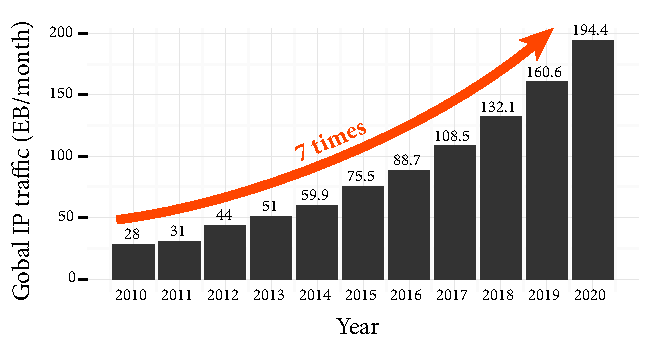
\includegraphics[width=7.5cm]{figures/vni.pdf}
    \vspace{-5pt}
    \caption{Global IP traffic~\cite{index2014forecast}.}
    \label{fig:vni}
\end{wrapfigure}
launched Amazon Snowball\index{Amazon Web Services (AWS)!Snowball}, a portable ready-to-be-shipped appliance with a storage capacity of 50~TB that can accommodate transfers of several Petabytes to \acrshort{aws}. These offloading techniques intend to overcome the challenges resulting from large-scale data transfers such as high network costs, long transfer times, and security concerns.

% As a reference, we give the duration to transfer 50~TB of data using typical Internet connections in Table~\ref{tab:truck-full-of-drives}. 
%In this thesis, we present a problem of scale. 
In this thesis, we propose to equip private vehicles with storage devices with the purpose of turning the road network into a large capacity transmission system. A back-of-the-envelope calculation shows that 10\% of the vehicles traveling the roads of France equipped with a 1~TB hard drive can transport up to 115~EB per day (1.3~PB per second). Extending this idea to the 1.2~billion cars available worldwide, the everyday mobility of vehicles represents an untapped potential for addressing the oncoming data tsunami. With data-intensive applications such as high-definition video, autonomous vehicles, and virtual reality, the demand for network bandwidth grows by an estimated 22\% per year. Already the case in some situations, in the next few years, the data consumption will outpace the network improvements made by providers in laying high-capacity fiber and speeding up their already-existing network infrastructure and servers~\cite{hecht2016bandwidth}. As shown in Figure~\ref{fig:vni}, the demand for bandwidth is at its strongest today: global \acrshort{ip} traffic has grown threefold during the past six years and is expected to double within the five next years~\cite{index2014forecast,gantz2012digital}.

The opportunistic use of vehicles follows the current trend of services that take advantage of the sharing economy (or access economy), such as BlaBlaCar and Uber, by enabling peer-to-peer-based sharing of goods and services. In our case, \textit{the trips made by the vehicles are shared resources we use to transport data on behalf of content providers}. 

Equipping vehicles with data storage also follows the second trend which consists in building value-added services right into an existing business. Examples of this trend include parcel delivery services built on top of existing passenger transportation services. In particular, Greyhound offers such a service that ``piggybacks'' on the trips made by buses as a part of the coach service.\footnote{\url{http://www.shipgreyhound.com/}} In the same manner, Uber proposes UberRUSH, an on-demand delivery service that relies on the fleet of Uber vehicles normally dedicated to passengers transportation.\footnote{\url{https://rush.uber.com}} In our case, private vehicles transport data for the account of content providers in exchange for their normal routine (\eg to synchronize backup data between remote data centers they operate). A service provider is then in charge of supervising the offloaded transfers then charged to the content providers and providing incentives to the vehicle owners for the data they transport (\eg through a ``get paid to drive'' program).
%% pourquoi pas uberEATS?

\begin{displayquote}
\textit{In this thesis, we characterize and exploit the existing mobility of everyday entities to mitigate or remove the limitations of conventional data networks. We rethink the design of popular services such as bulk data transfers or cloud-like file sharing by limiting or removing their reliance on such networks.
}\end{displayquote}
% \begin{mybox}[Vision of the thesis]{mybox:vision}
% In this thesis, we characterize and exploit the existing mobility of everyday entities to transport data for the account of large-scale services for end-to-end data transfers, storage and sharing, and vehicular resource virtualization.
% \end{mybox}


\section{Vision and data offloading design}

\begin{figure}[t]
   \centering
   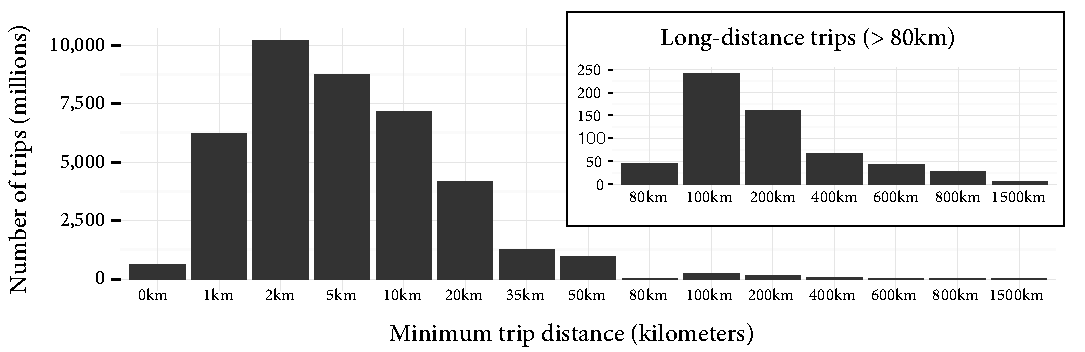
\includegraphics[width=0.9\textwidth]{figures/entd.pdf}
   \caption{Distribution of trips by distance travelled by vehicles in France. Source: the French National Household Travel Survey (ENTD), 2008~\cite{ENTD}.}
   \label{fig:entd}
\end{figure}

We exploit the \textit{delay-tolerance} of background traffic to offload bulk data transfers from a conventional data network such as the Internet over the road network. We target data transfers in the context of applications with a delay tolerance of several days (\eg distribution of large scientific datasets or traffic resulting from maintenance and provisioning activities of large-scale distributed systems)~\cite{laoutaris2009delay}. As noted by Hecht, the synchronization of the private content between remote data centers is one of the biggest drivers of bandwidth demand~\cite{hecht2016bandwidth}. Our data offloading takes opportunistic advantage of the increasing number of vehicular trips to physically transport data between locations~\cite{le2010mobilite}. 

One simple realization of the data offloading is to rely on the vehicles making the trip all the way from the source to the destination of a data transfer. However, as shown in Figure~\ref{fig:entd}, less than 1.4\% of the trips made by vehicles in France are longer than 80~km. While this number is still significant for short-distance data transfers (it corresponds to about 600 million trips per year), it becomes very low when the distance increases. Moreover, the number of destinations also increases with the distance of the trip, which results in just a few trips to transfer data over large distances. An alternative consists in using a dedicated fleet of vehicles acting as \textit{ferries} to transport the data from its source directly to its destination. However, this solution is costly and does not scale when the number of transfers increases, as more vehicles are needed to deliver the data.

Instead, we rely on dedicated facilities to \textit{compose} several flows of storage-enabled vehicles traveling in different directions. We refer to these facilities as \textit{offloading spots}\index{offloading spot} as we depict in Figure~\ref{fig:offloading-service-architecture}. Offloading spots are equipped with dedicated storage to temporarily store data and pass it between vehicles belonging to different flows. They are placed where vehicles stop often and long enough to transfer large amounts of data. Examples of such locations are on-street parking spots, garage parking, gas and electric charging stations, or supermarket parking lots. 

% When a vehicle stops at an offloading spot, the offloading spot decides whether to load or unload data based on the future direction of the vehicle. While this information may raise some privacy concerns for the driver and the passengers, we assume that it is derived from the positioning system onboard the vehicle, which provides the historical trajectories and planned itinerary to accurately predict the future direction of the vehicle~\cite{krumm2006predestination}.



%The offloading spots serve two distinct purposes, depending on their relative position in the offloading process. We represent the dual role of the offloading spots in Figure~\ref{fig:offloading-service-architecture}, in the context of a large-scale transfer of delay-tolerant data between two remote data centers. Part or all of the data originating from a conventional data network is first \textit{transloaded}\index{transloading} to the closest edge offloading spot. The data is temporarily stored at the offloading spot and is loaded onto the stopping vehicles. Subsequent intermediate offloading spots act as data relays where data is \textit{transshipped}\index{transshipping}. Vehicles drop off the data they carry while they stop at the offloading spot. The data is temporarily stored until subsequent vehicles pick it up and carry it to the next offloading spot. Once at the destination, the data is finally transloaded back into the conventional data network.

\begin{figure}[t]
    \centering
    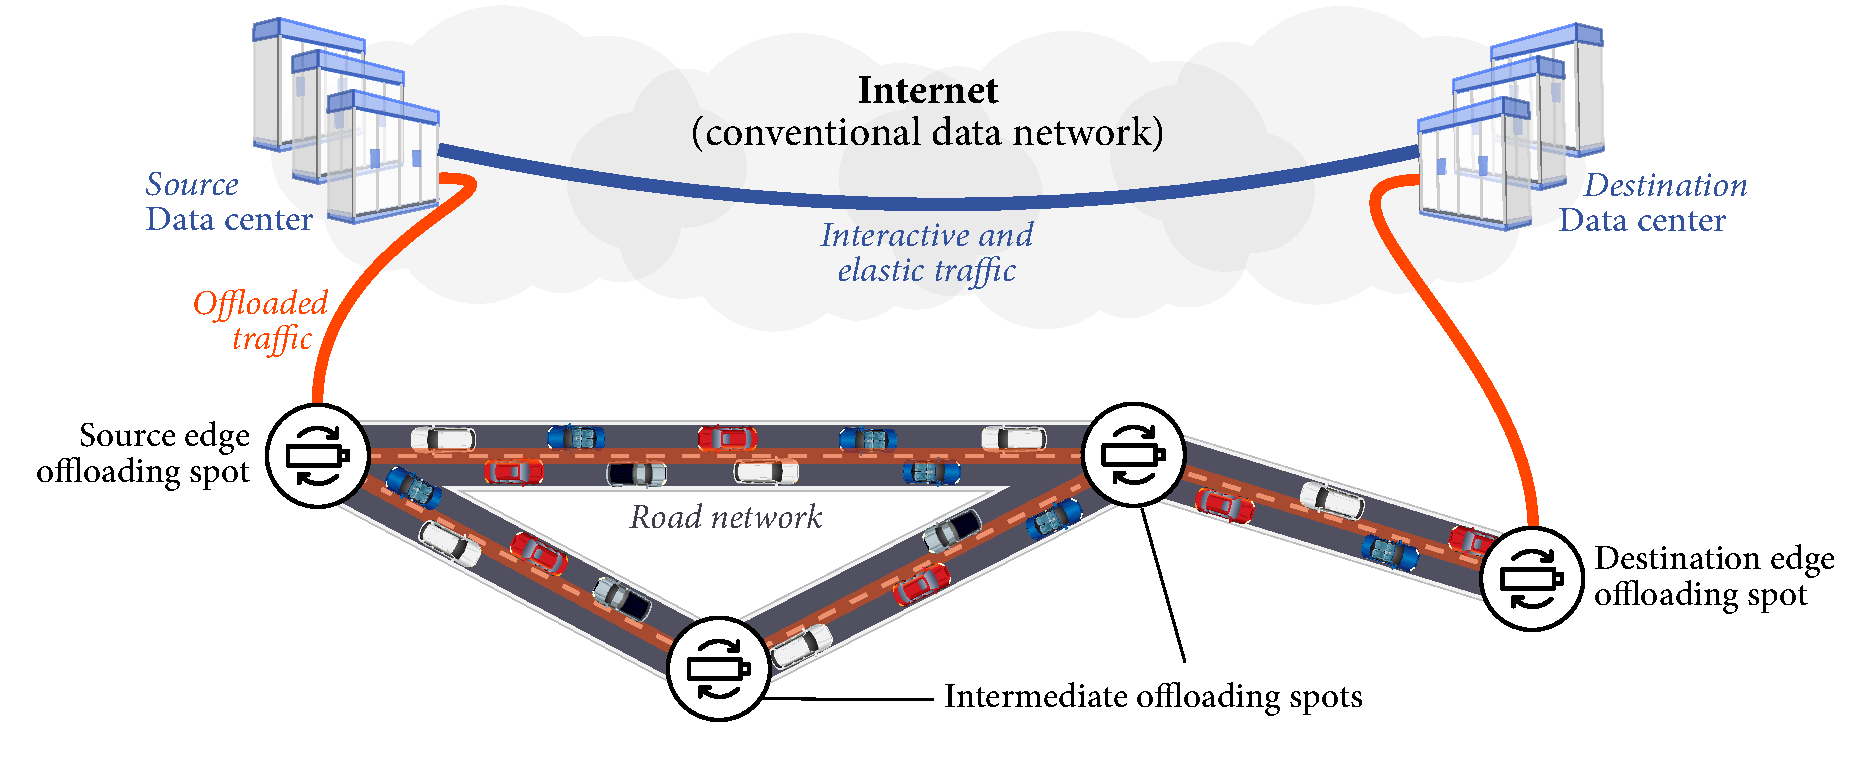
\includegraphics[width=0.9\textwidth]{figures/architecture-2.pdf}
    \caption{General overview of the data offloading we propose in this thesis.}
    \label{fig:offloading-service-architecture}
\end{figure}

% Offloading spots can also be as locations where segments of trajectories made by independent vehicles are concatenated into a single logical path followed by the offloaded data. The storing capabilities of offloading spots allow the data to be passed asynchronously from one vehicle to another. 
Following up on the work on traffic offloading, we extend the concept of offloading spot according to two distinct directions both in the context of vehicular cloud services. In the first extension, we leverage the storage capacity of the offloading spots to turn them into repositories and provide a geo-distributed system to store and share files of mobile users. To enforce the file sharing, we rely on the movements of vehicles traveling between the offloading spots to replicate the files and make them accessible to the mobile users. In the second extension, we virtualize the resources of the vehicles to create a virtual vehicular network. We dematerialize the offloading spots into pre-defined areas that feature high densities of vehicles to enable transfers of virtual machines between the vehicles. With these extensions, we further show that the existing mobility of vehicles has the potential to provide cloud services with limited reliance on conventional data networks.

% In the first extension, we leverage the storage capacity of the offloading spots to provide a cloud-like storage and sharing system for mobile users in an urban environment. The offloading spots act as repositories where users first upload their files, which are then replicated among the other repositories using the movements of the mobile users between the repositories. The replication increases the likelihood of processing the user requests to store or retrieve a file in a timely fashion.  

% In a second extension, we dematerialize the offloading spots into pre-defined areas that feature high densities of vehicles and where contacts between vehicles last long enough to transfer large amounts of data. We exploit these areas in the context of the virtualization of a vehicular network operating in an urban environment. Each vehicle hosts one or many virtual machines exploiting the abstraction provided by virtualizing the vehicle resources.
%We virtualize the resources embedded in the vehicles (\ie compute, storage, and sensing) into virtual machines. The virtualized resources are allocated to service providers, who deploy services that benefit from the movements and the shared resources of the vehicles, such as a large-scale sensing platform. 
% We show the benefits of dematerializing the offloading spots when
%and the \acrlong{v2v} communications happening in these areas 
% the migration of virtual machines is required as a result of changes in the physical topology or reallocations of the virtual resources.

%We explore \textit{how to enable efficient and reliable data transfers over the road network}. We propose an architecture that relies on a centralized controller to allow flexible and scalable configuration of the offloading spots. We use the \acrfull{sdn}\index{Software-Defined Networking (SDN)}~\cite{mckeown2008openflow} paradigm, which provides the logistics for efficient and effective vehicular transportation of data. Our \acrshort{sdn}-controlled architecture consists of a central controller\index{controller} and a collection of offloading spots. The controller receives demands to offload data transfers onto the road network. An offloading demand\index{offloading demand} indicates both the source and destination of the transfer and performance requirements, such as delay and bandwidth. The controller is then in charge of mapping the offloading demands onto sequences of offloading spots by allocating the corresponding data transfers to vehicle flows traveling between the offloading spots. 

\section{Challenges}

Firstly, we need to efficiently allocate data transfer demands to the existing flows of vehicles. We refer to this problem as the \textit{vehicle flow allocation problem}. To solve it, we need to design an efficient allocation process of the data transfers that optimizes target performance metrics, while matching the performance requirements of the corresponding demands.

\begin{wrapfigure}[13]{o}[0.7\marginparwidth]{6.2cm}
    \vspace{-15pt}
    \centering
    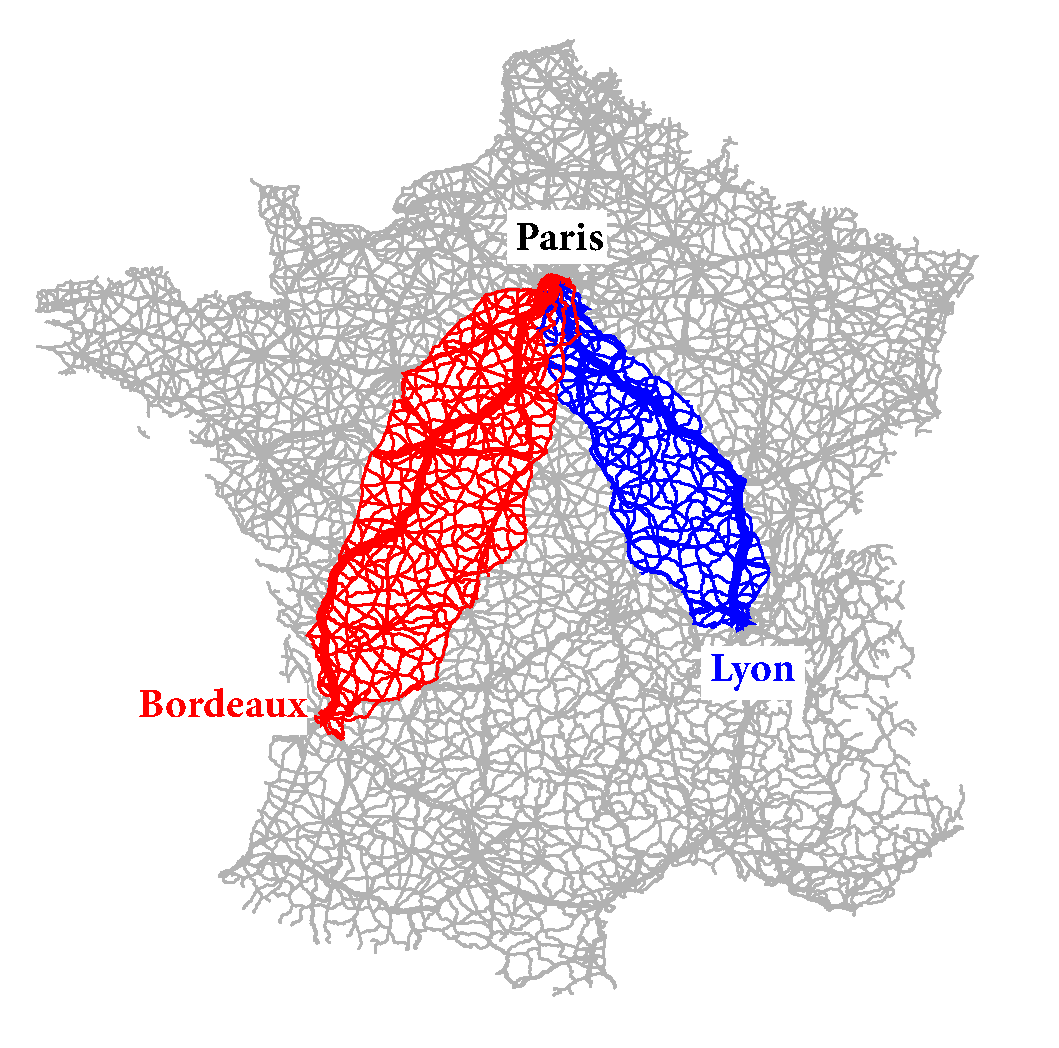
\includegraphics[width=6cm]{figures/france-roads-2.pdf}
    \caption{Main roads connecting Paris to Lyon and Bordeaux.}
    \label{fig:paris-lyon}
\end{wrapfigure}
Secondly, we need to cope with the scale of the road network in order to achieve a scalable and efficient vehicular data offloading. The complexity of the road network's topology and the large number of vehicular trips both make the vehicle flow allocation problem computationally intractable. We illustrate the need for a scalable allocation mechanism in Figure~\ref{fig:paris-lyon}, where we depict the routes of the potential trips that can be allocated to offload transfers originating from Paris to Bordeaux and Lyon. 

Finally, we need to ensure reliable data transfers. Since vehicles may fail to deliver the data they carry to the next offloading spot or the final destination, we need to rely on and adapt techniques to recover from the data losses.

In the extensions of our main work, the underlying challenge is to determine the locations of the offloading spots, whether they are materialized or not, according to the specific requirements of the services we deploy. 

In our vehicular file sharing system, we need to design an algorithm to place the repositories at strategic locations where they can capture a maximum number of user requests before they expire, while connecting them together by the movements of the users to enable the replication. In our virtual vehicular network, we need to identify the location of the areas where vehicles meet frequently and long enough to transfer large amounts of data, such as virtual machines.



\section{Contributions and thesis outline}

\paragraph{First contribution: Survey and taxonomy of techniques to transfer data using everyday mobility (Chapter~\ref{cha:state-of-the-art}).}

We begin this thesis by providing an exhaustive survey and taxonomy of the existing techniques that help exploit the mobility of everyday entities to transport data in the context of various applications. We categorize the existing techniques based on whether the delivery involves a single entity or multiple entities that take turns to transport the data. We also describe the various approaches proposed in the literature for characterizing the mobility and controlling the data forwarding.\\[3pt]
%that we use in the following chapters to achieve massive data offloading. \\
\textit{Related paper}:
\begin{itemize}
    \item Benjamin Baron, Prométhée Spathis, Marcelo Dias de Amorim, and Yannis Viniotis. ``Data transfers using everyday mobility: A survey.'' Submitted to \textit{IEEE Communications Surveys \& Tutorials}, 2016.
\end{itemize}


\paragraph{Second contribution: Assessment of the vehicular offloading concept (Chapter~\ref{cha:feasibility-study}).}

In Chapter~\ref{cha:feasibility-study}, we assess the concept of vehicular data offloading. We compare the cost of transferring data using the existing mobility of vehicles to the cost of transferring the same amount data on the Internet. We first introduce a map reduction procedure which mitigates the complexity of the road network. The output of this procedure is a logical representation which translates and characterizes the flows of vehicles into network quantities. This representation is used to solve an allocation procedure which selects the flows of vehicles in charge of carrying the offloaded data. We formulate and solve this allocation procedure as a \textit{revenue maximization model}\index{vehicle flow allocation problem!revenue maximization model} that allocates the flows of vehicles so as to maximize the cost-benefit of offloading data on the road network compared to data transfers over conventional data networks.
%We use replication techniques at the offloading spots to recover from data losses. 
Finally, we show using actual traffic counts for the French road network that our offloading concept can achieve an aggregate capacity in the Petabyte range per week.\\[3pt]
\textit{Related papers}:
\begin{itemize}
    \item Benjamin Baron, Prométhée Spathis, Hervé Rivano, and Marcelo Dias de Amorim. ``Offloading massive data onto passenger vehicles: Topology simplification and traffic assignment.'' \textit{IEEE/ACM Transactions on Networking}, 2015.
    \item Benjamin Baron, Prométhée Spathis, Hervé Rivano, and Marcelo Dias de Amorim. ``Vehicles as big data carriers: Road map space reduction and efficient data assignment.'' \textit{IEEE Vehicular Technology Conference (VTC Fall)}, 2014.
    \item Benjamin Baron, Prométhée Spathis, Hervé Rivano, and Marcelo Dias de Amorim. ``Étude de l'intermodalité pour le délestage des réseaux d'infrastructure.'' \textit{Algotel 2015~---~17èmes Rencontres Francophones sur les Aspects Algorithmiques des Télécommunications}, 2015.
\end{itemize}


% \paragraph{Second contribution: Road network logical abstraction (Chapter~\ref{cha:vehicular-offloading-service}).}

% Based on the models of the literature that characterize the mobility of the entities, we propose a reduction of the road map space into a logical overlay network. In Chapter~\ref{cha:vehicular-offloading-service}, we introduce the \textit{offloading overlay}\index{offloading overlay}, which mitigates the complexity of the road network and translates its attributes into network quantities. Together with a centralized architecture with a controller that has a holistic view of the system, it allows efficient allocation of data transfers on the road resources. We evaluate the benefits of the centralized architecture and the offloading overlay in the context of electric vehicles with a concrete deployment plan of charging stations on the French roads. \\
% \textit{Related papers}:
% \begin{itemize}
%     \item Benjamin Baron, Prométhée Spathis, Hervé Rivano, and Marcelo Dias de Amorim. ``Offloading massive data onto passenger vehicles: Topology simplification and traffic asssignment.'' \textit{IEEE/ACM Transactions on Networking}, 2015.
%     \item Benjamin Baron, Prométhée Spathis, Hervé Rivano, Marcelo Dias de Amorim, Yannis Viniotis, and Mostafa Ammar. ``Data haulage: Efficient resource management on the road network.'' Submitted to \textit{IEEE Transactions on Network and Service Management}, 2016.
% \end{itemize}


\paragraph{Third contribution: Offloading infrastructure centralized control (Chapter~\ref{chap:implementation}).}

We propose an architecture that implements the concept of vehicular data offloading. We rely on a centralized architecture that enables efficient control of the offloading infrastructure. This architecture consists of a controller and the collection of offloading spots acting as forwarding engines. The controller is in charge of selecting the road network path for each offloading demand it receives. The selection of road network paths is done so as to maximize the throughput of the resulting transfer while ensuring the fair allocation of flows of vehicles traveling the paths among the other transfers that allocated to the same paths. This is achieved by modeling and solving the allocation of a data transfer to a road path according to a max-min fairness problem\index{vehicle flow allocation problem!max-min fair allocation model}. 
%This problem that maximizes the resulting throughput while ensuring the fair allocation of the data transfers. 
%and consisting of the sequence of offloading spots. We introduce this architecture and we formulate the data transfer allocation problem as a max-min fairness allocation problem\index{data transfer allocation problem!throughput maximization model} that maximizes the resulting throughput while ensuring the fair allocation of the data transfers. 
The controller translates the output of the allocation of a data transfer by a set of forwarding rules installed at the offloading spots composing the selected road network.  Finally, the controller ensures the reliability of the offloaded data using redundancy and retransmission techniques. %to recover data lost by vehicles failing to deliver data to the next offloading spot. 
With simulations on the French road network and elaborated traffic modelling techniques presented in the Appendix~\ref{cha:traffic-forecasting-techniques}, we show that the offloading architecture we propose has the potential to offload several Petabyte of data per day.\\[3pt]
\textit{Related papers}:
\begin{itemize}
    \item Benjamin Baron, Prométhée Spathis, Hervé Rivano, Marcelo Dias de Amorim, Yannis Viniotis, and Mostafa Ammar. ``Data Haulage: Efficient resource management on the road network.'' Submitted to \textit{IEEE Transactions on Network and Service Management}, 2016.
    \item Benjamin Baron, Prométhée Spathis, Hervé Rivano, Marcelo Dias de Amorim, Yannis Viniotis, and Joseph Clarke. ``Software-defined vehicular backhaul.'' \textit{IFIP Wireless Days (WD)}, 2014.
\end{itemize}


\paragraph{Fourth contribution: Vehicular cloud services (Chapter~\ref{cha:vehicular-cloud-services}).}

We propose two extensions to the work we conduct in traffic offloading. We extend the concept of offloading spots in the context of two vehicular cloud services. A first service turns the offloading spots as repositories where mobile users can upload and share files. We propose a placement algorithm derived from the Maximal Covering Location Problem~\cite{church1974maximal} that determines the location of a target number of repositories such that (\textit{i}) a maximum of users are covered before their uploading or retrieval requests expire and such that (\textit{ii}) the synchronisation of the repositories can be done by using the existing movements of the users.

The second service virtualizes the resources of vehicles operating within a large mobile network. The offloading spots refer to specific areas where the virtual machines exploiting the abstract representation of the vehicle resources can migrate between vehicles while in contact. We propose a methodology for analyzing the spatial distribution of the contact density. This methodology determines the specific areas where contacts are long and frequent enough to accommodate the migration of virtual migrations.\\[3pt]
\textit{Related papers}:
\begin{itemize}
    \item Benjamin Baron, Miguel Campista, Prométhée Spathis, Luís Henrique MK Costa, Marcelo Dias de Amorim, Otto Carlos MB Duarte, Guy Pujolle, and Yannis Viniotis. ``Virtualizing vehicular node resources: Feasibility study of virtual machine migration.'' \textit{Elsevier Vehicular Communications}, 2016.
    \item Benjamin Baron, Prométhée Spathis, Marcelo Dias de Amorim, and Mostafa Ammar. ``Cloud storage for mobile users using pre-positioned 
    storage facilities.'' \textit{ACM SmartObjects}, 2016.
\end{itemize}

\paragraph{Thesis outline.}
This manuscript is organized in six chapters, including this introduction (Chapter~\ref{cha:introduction}). Chapter~\ref{cha:state-of-the-art} presents a review of previous approaches that propose to use mobility of entities to transport data. The two following chapters~\ref{cha:feasibility-study} and \ref{chap:implementation} present the main contribution of the thesis with, respectively, a revenue analysis and a practical implementation of the vehicular data offloading system. Chapter~\ref{cha:vehicular-cloud-services} presents two extensions of the data offloading system for vehicular cloud services. Each chapter begins with a brief introduction followed by a list of the main contributions. Given the novelty of our work, we provide additional discussions for each chapter on related topics we chose not to address in detail, including data security, privacy concerns, and road traffic dynamics. Finally, we conclude this thesis with a last chapter (Chapter~\ref{cha:conclusion}) that summarises our work and a raises futher questions as a plan for future research. 

\paragraph{Collaborations.} 
The research presented in this thesis was conducted in the context of a number of scientific collaborations: Hervé Rivano (Inria), Yannis Viniotis (NCSU and Cisco), Joe Clarke (Cisco), Miguel Campista (UFRJ), Luís Henrique MK Costa (UFRJ), Otto Duarte (UFRJ), Guy Pujolle (UPMC), and Mostafa Ammar (Georgia Tech).